\section{Jets in ATLAS}
\label{sec:Det:Jets}

The jet definition within ATLAS uses the \antikt{} algorithm, which is described in Section \ref{sec:Theory:Jets}. 
This algorithm groups related energy deposits in the ATLAS calorimeters.
Different input objects can be used with the \antikt{} algorithm, such as cells, towers and topoclusters and these objects can be calibrated to different energy scales.
In this analysis, unless otherwise stated, the jets are defined using the \antikt{} algorithm with a distance parameter of 0.6 running over topocluster at EM scale, where topoclusters and EM scale are defined in Section \ref{sec:Det:Calo}.


\subsubsection{Jet Energy Scale (JES)}

The jet response needs to be calibrated to take into account both detector and physics responses such as dead material, particle being bent into and  out of the jet, and noise threshold variation. 
Also, jets are found using EM-scale topoclusters and need to be calibrated due to the non-compensation of the hadronic calorimeter which has a lower detector response to hadrons than to EM deposits.
An EM+JES calibration was determined as a function of the jet \pt{} and rapidity to account for these effects.

The EM+JES calibration was done in three consecutive corrections.
The first was a pile-up offset correction designed to subtract energy contributions due to additional $pp$ interactions.
The correction is presented in \cite{ref:OffsetCorrection}, where the average energy in towers is considered as a function of $\eta{}$, the number of primary vertices and the bunch spacing.
The second correction was the vertex correction, which defined the origin of the jets to be the primary vertex.
This correction changes the direction and \pt{} of the jet, but not the energy, and it improves the angular resolution of the jet.
The original uncorrected $\eta{}$ is defined as the detector $\eta$.
The final correction is the jet energy scale (JES) correction.

The JES correction uses fully simulated MC, ``reco'', jets and jets at hadron level, ``truth'' jets, to obtain correction factors as a function of jet energy and jet rapidity. 
The response of the calorimeter to jets can be defined using these fully simulated MC samples as
\begin{equation}
\mathcal{R(\eta)} = \frac{\pt{}^{reco}(\eta)}{\pt{}^{truth}(\eta)}
\label{JetPerf:MCJetResp}
\end{equation}
where \pt{}$^{reco}$ is the \pt{} of the MC jet after full simulation of the detector, and  \pt{}$^{truth}$ is the \pt{} of the MC jet at hadron level.
The truth and reco jets are matched using a \dr{} requirement of 0.3.
The correction factors are calculated as a function of the jet's detector $\eta$ opposed to the vertex corrected $\eta$, as they represent calibrations for different detectors, and also as a function of the energy, as the detector responds to energy. 
Figure \ref{Det:MCResp} shows the jet responses, at EM scale, as a function of detector $|\eta|$ for different jet energies. 
From the comparison between fully simulated MC jets and truth jets, a small correction on the jet rapidity is calculated. 
This is due to part of jets falling into regions with lower response, giving a $\eta$ shift towards the higher responding areas. 
The original derivation of these factors can be found in \cite{ref:OffsetCorrection,ref:JES,ref:JES_basic}.

\begin{figure}
\centering
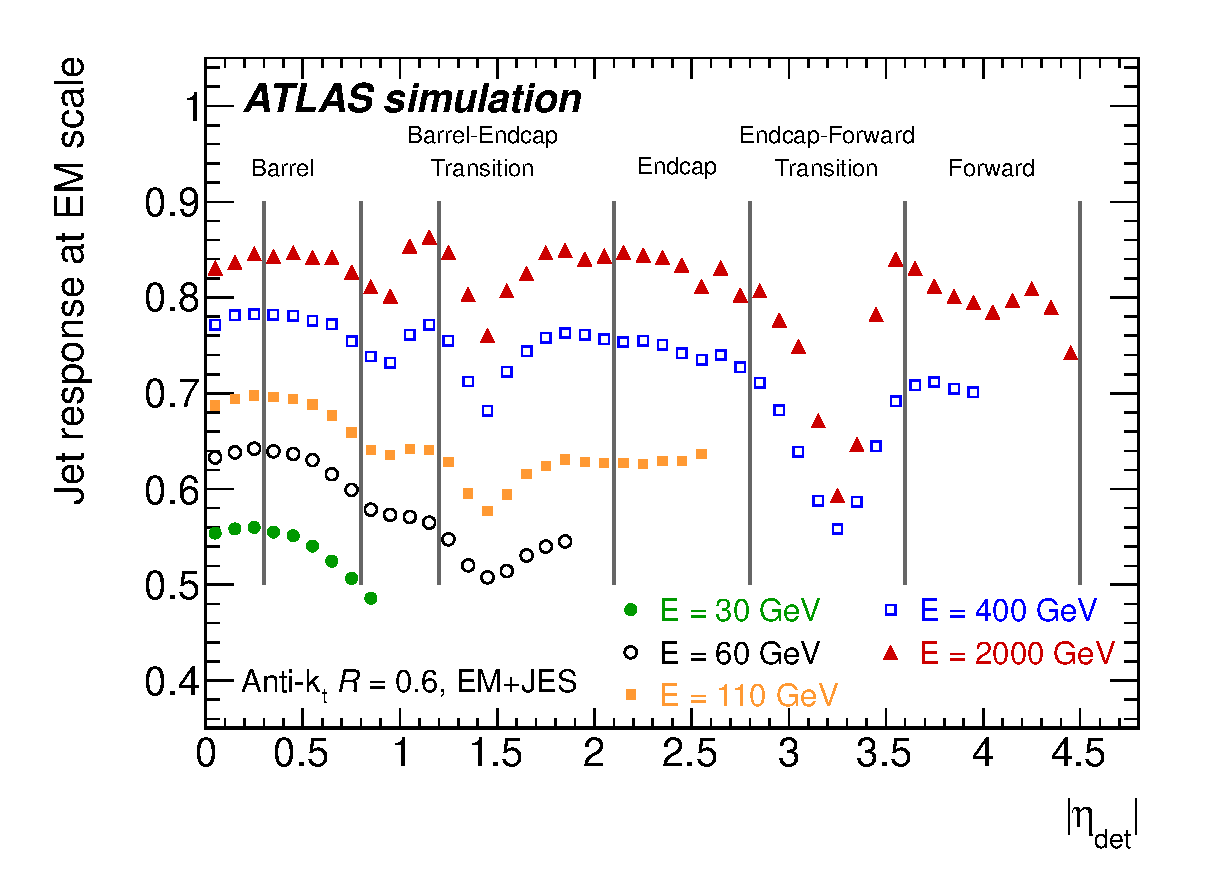
\includegraphics[width=0.8\textwidth]{figures/Detector/JetCalibfig_JES_vs_eta_Binning.eps}

\caption[Jet response for different regions of the ATLAS calorimeter]{ 
PYTHIA simulated jet EM-scale response as a function of reconstructed jet detector $\eta$ for different jet energies \cite{ref:JES}.
The different evaluated regions are shown, as well as their relation to the detector geometry. 
\label{Det:MCResp}
}
\end{figure}


\subsubsection{Jet Energy Scale Uncertainty}

The EM+JES method of calibration is based primarily on the ability of the MC to correctly simulate the ATLAS detector and also to model the physics effects such as energy flow out of the jet.
In-situ methods are used to validate the JES calibration and assign an uncertainty.
The JES uncertainty is derived from in-situ data measurements and also by varying MC settings. 
It is determined by combining the non-closure of the EM+JES on fully simulated MC jets, calorimeter response to isolated hadrons using test-beam information and in-situ methods, additional detector material, noise thresholds, differences compared to other MCs, uncertainties due to pile-up and \pt{} balance of dijet events. 


\begin{figure}
\centering
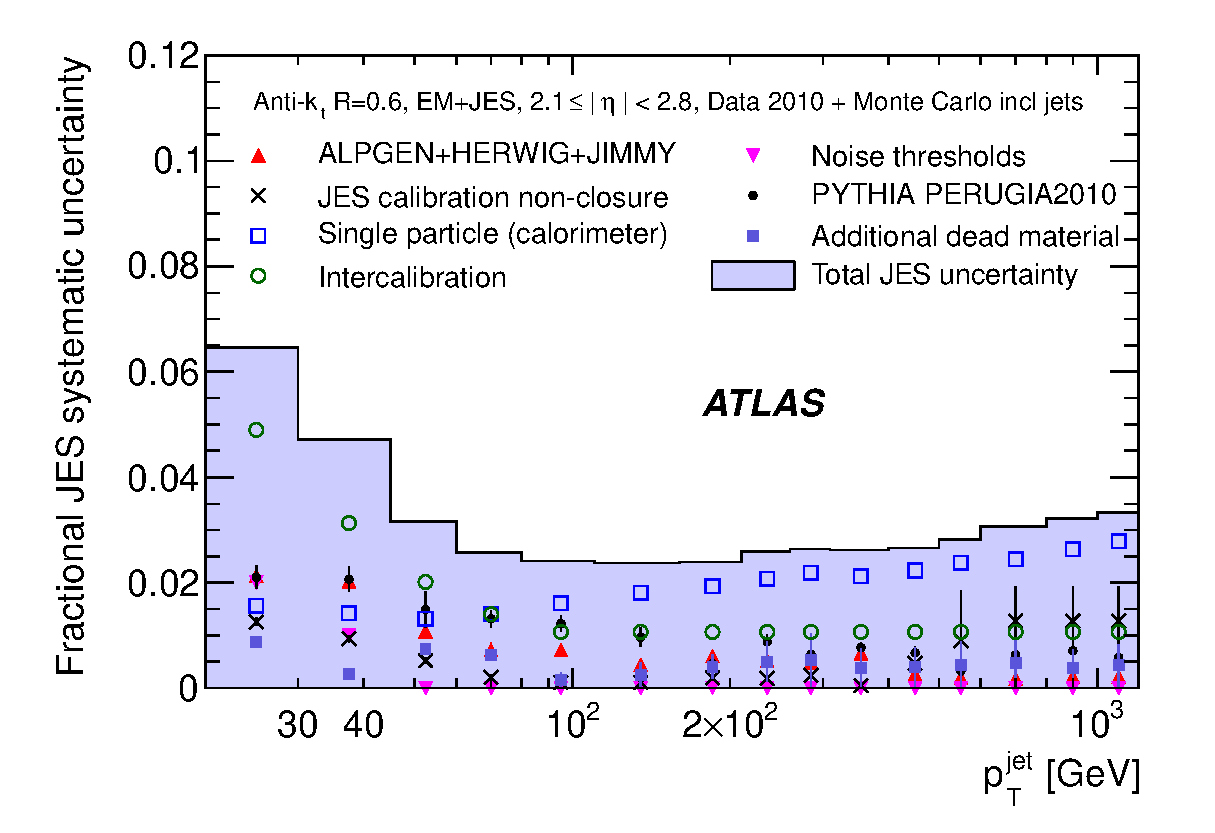
\includegraphics[width=0.8\textwidth]{figures/Detector/JESSummary_JESUncertainty_AntiKt6Topo_EMJES2.1-2.8.eps}
\caption[JES Uncertainty]{ 
Fractional JES uncertainty for jets with $2.1\le|\eta|\le2.8$ as a function of the jet \pt{} \cite{ref:JES}. 
\label{Det:JESU}
}
\end{figure}

Figure \ref{Det:JESU} shows the fractional JES uncertainty for jets with $2.1\le|\eta|\le2.8$ as a function of the jet \pt{}.
The dominant systematic at high \pt{} is the single particle response which comes from test-beam single pion information and the calorimeter response for a single hadron.
At low \pt{}, dijet balance (intercalibration) is the most significant uncertainty.
Dijet balance is an in-situ method of extending the uncertainty in the central region to other regions of the detector, and will be discussed in more detail in Chapter \ref{chp:JetPerf}.


\subsubsection{Jet Energy Resolution}

The jet energy resolution (JER) is a measure of the expected range of measured jet \pt{} compared to the original object. 
Some causes of the fluctuations in the measurement of a jet \pt{} are different hadron/EM contributions, non-average amount of additional energy from pile-up, and statistical fluctuations in the sampling technique across multiple calorimeter layers.
The JER was determined using the bi-sector method and the \pt{} balance of dijet events described in \cite{ref:JER,ref:JER2}. 




\subsubsection{Jet Cleaning}

Jets produced in an event need to be discriminated from ``bad'' background jets that come from  signal spikes in cells within the HEC and EM noise in the calorimeter, cosmic rays or non-collision background.
Table \ref{det:Cleaning} shows the loose and medium cleaning requirements used to remove the bad jets where
\begin{itemize}
  \item The jet charge fraction, $\mathbf{f_{CH}}$, is the ratio of the sum of the \pt{} of tracks associated to the jet to the calibrated jet \pt{};
  \item  $\mathbf{f_{EM}}$ is the fraction of the jet EM scale energy that comes from EM clusters;
  \item  $\mathbf{f_{HEC}}$ is the fraction of the jet energy that was measured in the HEC;
  \item The LAr quality, $\mathbf{Q_{LAr}}$, is the fraction of the jet energy coming from LAr cells with poor signal shape quality;
  \item The HEC quality, $\mathbf{Q_{HEC}}$, is the fraction of the jet energy coming from HEC cells with poor signal shape quality;
  \item \Bold{neg. E} is the sum of the negative energy cells in the jet;
  \item Jet time, \Bold{t}, is the mean time between the cells in the jet and the event time;
  \item $\mathbf{f_{max}}$ is the maximum energy fraction in one calorimeter layer.
\end{itemize}

Jets coming from HEC spikes have most of the energy coming from a single noisy calorimeter cell, and so a $f_{HEC}$ requirement is applied to ensure energy deposits outside the HEC form a significant part of the total energy.
Fake jets coming from EM coherent noise are removed by cutting on the fraction of EM energy.
Finally, jets from non-collision backgrounds and cosmic rays are removed using a combination of timing and energy layer requirements.

The loose cleaning requirements are defined to have an efficiency of greater than 99\% for good jets, but a fraction of bad jets still remain. 
Whilst the medium cleaning requirements remove a higher proportion of bad jets, they have inefficiencies at low \pt{} for good jets. 

While the bad jets do not come from energy deposits from the interaction, there is a subset of jets, called ``ugly'' jets, which are energy deposits from the interaction which have been badly measured. 
Ugly jets are often found in regions between detectors, ``cracks'' regions, where the performance of the detectors are not optimal.
Two selection criteria are applied to remove ugly jets.
First, the jet energy which falls into the transition between the barrel and the end-cap is required to be less that half the total jet energy.
Second, the fraction of energy that comes from bad cells inside the jet is required to be less than half of the total jet energy.


\begin{table}
\begin{center}
\footnotesize

\begin{tabular}{|c||c|c|}
\hline
& Loose & Medium = Loose OR \\
\hline
            & $\rm f_{HEC}<0.5$ \& $|\rm Q_{HEC}|>0.5$                         &                                                              \\
HEC spikes  &              or                                              & $\rm f_{HEC}>1-|Q_{HEC}|$                                          \\
            &  $\rm |neg.E|>60$ GeV                                        &                                                              \\
\hline
EM          &                                                              &                                                              \\
coherent    & $\rm f_{EM} >0.95$ \& $\rm |Q_{LAr}| >0.8$ \& $|\eta|<2.8$     &   $\rm f_{EM} >0.9$ \& $\rm |Q_{LAr}| >0.8$ \& $|\eta|<2.8$    \\
noise       &                                                              &                                                              \\
\hline
            &           $\rm |t|>25$ ns                                                    &                                                              \\
Non-        &              or                                              &  $\rm |t|>10$ ns                                          \\
collision   & $\rm f_{EM} <0.05$ \& $\rm f_{CH}<0.05$ \& $|\eta|<2$     &   or     \\
background  &        or                     &   $\rm f_{EM}<0.05$ \& $\rm f_{CH} <0.1$ \& $|\eta|<2$    \\
\& cosmics  & $\rm f_{EM} <0.05$ \&  $|\eta|>2$     &   or     \\
            &        or                     &   $\rm f_{EM}>0.95$ \& $\rm f_{CH} <0.05$ \& $|\eta|<2$    \\
             & $\rm f_{max}<0.99$ \&  $|\eta|<2$     &        \\

\hline

\end{tabular}
\caption[Jet Cleaning Definitions]{
Loose and Medium jet cleaning definitions.
\label{det:Cleaning}
}
\end{center}
\end{table}


